%!TeX spellcheck = en_UK
% Die erste (unkommentierte) Zeile im Dokument legt immer die
% Dokumentklasse fest
\documentclass{scrartcl} 

% Präambel:
% Einbinen von zusätzlichen Paketen. Falls für eine Datei keine Endung
% explizit angegeben wird, benutzt LaTeX '.tex'. Im Folgenden wird
% also die Datei 'edv_pakete.tex' eingebunden.
% Die erste Zeile im Dokument legt immer die Dokumentklasse fest
%\documentclass[notitlepage]{scrreprt}
    % Die wichtigsten Dokumentklassen:
    %   scrbook, scrreprt, scrartcl, beamer, standalone
    % Einige gängige Optionen für \documentclass:
    %   ngerman
    %   titlepage, notitlepage
    %   onecolumn, twocolumn
    %   oneside, twoside
    %wird in Hauptdatei festgelegt

% Präambel

% Einige KOMA-Script-Optionen
\KOMAoptions{fontsize=12pt,paper=a4}      %Schriftgröße, Papierformat
\KOMAoptions{DIV=11}                      % Parameter mit dem man den Seitenrand ändern kann
\KOMAoptions{listof=totoc}

% Hier werden einige Pakete eingebunden
\usepackage[utf8]{inputenc}               % Direkte Eingabe von ä usw. Input=Eingabe
\usepackage[T1]{fontenc}                  % Font Kodierung für die Ausgabe Font=Ausgabe
\usepackage[english]{babel}               % Verschiedenste sprach-spezifische Extras, ngerman für neue deutsche Rechtschreibung, auch UK oder US möglich
\usepackage[autostyle=true]{csquotes}     % Intelligente Anführungszeichen, arbeitet mit Babel zusammen
%

\usepackage{amsmath}%Mathedarstellung
\usepackage{commath}%Mathedarstellung
\usepackage{physics}%Physik-Symbole
%\usepackage{IEEEtrantools}%IEEEeqnarray
%
\usepackage{siunitx}   % Intelligentes Setzen von Zahlen und Einheiten
%\sisetup{locale = DE}  % Deutsch als locale für die Zahlen und Einheiten
%http://tex.stackexchange.com/questions/2291/how-do-i-change-the-enumerate-list-format-to-use-letters-instead-of-the-defaul

\usepackage{enumitem}%erlaubt u.A. die Aufzählung mit Buchstaben, gefunden auf http://tex.stackexchange.com/questions/2291/how-do-i-change-the-enumerate-list-format-to-use-letters-instead-of-the-defaul
%
\usepackage[varg]{txfonts}                % Schönere Schriftart, muss nach amsmath, damit keine Fehlermeldung kommt
\usepackage{graphicx} %einbinden von Figuren/Bildern
\graphicspath{{figs/}} % Stammverzeichnis der verwendeten Bilder, muss im selben Ordner wie Hauptdatei sein
%
\usepackage[backend=biber, style=numeric, sorting=none]{biblatex}
%Verwenden von \cite in \footnote: Bibliographie drucken lassen, mehrmals kompilieren
\usepackage{hyperref}%erzeugt klickbare Elemente
\usepackage[all]{hypcap}%hyperref-befehle springen zum oberen Rand des Bildes
% Zum Einbinden von Programmcode verwenden wir das listings-Paket
\usepackage{listings}

% Für Syntax-Highlighting:
\usepackage{xcolor}

\usepackage{longtable}

% Die folgenden listings-Einstellungen sind nötig, um
% deutsche Umlaute und die Tilde (~) in listings-Umgebungen
% verwenden zu können.
\lstset{
    basicstyle=\ttfamily,    
    literate={~} {$\sim$}{1} % set tilde as a literal
    {ö}{{\"o}}1
    {ä}{{\"a}}1
    {ü}{{\"u}}1
    {ß}{{\ss}}1
    {Ö}{{\"O}}1
    {Ä}{{\"A}}1
    {Ü}{{\"U}}1
}

% Farben für Code-Syntaxhighlighting und Weiteres festlegen:
\lstset{
    % Keine besondere Markierung für Leerzeichen in Codes
    showspaces=false,               
    showstringspaces=false,         
    % Farebn für Code-Kommentare und Schlüsselworte:
    commentstyle=\color{red},       % comment style
    keywordstyle=\color{blue},      % keyword style
    stringstyle=\color{orange},		% string style
    breaklines=true,
    numbers=left,                    % where to put the line-numbers; possible values are (none, left, right)
    numbersep=5pt,                   % how far the line-numbers are from the code
    stepnumber=5, 					%how often there are line numbers in code listings
    tabsize=4, 						%default tabsize set to 4 spaces
    %language=python,
    }
%gefunden auf https://en.wikibooks.org/wiki/LaTeX/Source_Code_Listings
%eigene Kommandos/Abürzungen
\newcommand{\tb}{\textbackslash}
\newcommand{\txt}{\texttt}
\newcommand{\umt}{u_{(i+i\%2)/2}^{(2a)}}
\newcommand{\utmt}{u_{(i-2+i\%2)/2}^{(2a)}}
\newcommand{\uti}{\tilde{u}_i^{(a)}}
\newcommand{\utio}{\tilde{u}_{i-1}^{(a)}}




% Verzeichnisse mit Abbildungen; kann gestrichen werden,
% falls Sie dies schon in edv_pakete.tex definiert haben:
%\graphicspath{{../report}}

\addbibresource{refs.bib} %Hinzufügen einer Literaturdatenbank aus dem angegebenen Verzeichnis

% Titel, Autor und Datum
\title{Computational Physics}
\subtitle{Exercise 7}
\date{\today}
\author{Christiane Groß, Nico Dichter}

% Jetzt startet das eigentliche Dokument
\begin{document}
	\maketitle
	
\section{Theory}

\subsection{Discretization of the Lippmann-Schwinger-equation}

Using some definitions given in the lectures and on the sheet, we are able to discretize the Lippmann-Schwinger-equation given on the sheet. we use Gauss-Legendre-integration and get the following matrix-equation:

\begin{longtable}{>{$\displaystyle}r<{$}>{$\displaystyle}c<{$}>{$\displaystyle}l<{$}}
	f(p'')&=&2\mu p''^2V_l(p, p'')t_l(p'', p')\\
	q&=&p_N\\
		
	V(p_i, p_j)&=&V_{ij}\\
		
		
	t(p_i, p_j)&=&t_{ij}\\
		
	\int_{0}^{\infty}\dd p'' g(p'')&=&\sum_{k=0}^{N-1}\omega_k g(p''_k)\\
	
	&&\\
	
	\dashint_{0}^{p_{max}}\frac{\dd p''}{q^2-p''^2}&=&\lim\limits_{\epsilon\to 0}\int_{0}^{q-\epsilon}\dd p''\frac{1}{(q+p'')(q-p'')}+\int_{q+\epsilon}^{p_{max}}\dd p''\frac{1}{(q+p'')(q-p'')}\\
	&=&\lim\limits_{\epsilon\to 0}\frac{1}{2q}\left(\int_{0}^{q-\epsilon}\dd p''\frac{1}{q+p''}-\frac{1}{p''-q}+\int_{q+\epsilon}^{p_{max}}\dd p''\frac{1}{q+p''}-\frac{1}{p''-q}\right)\\
	&=&\lim\limits_{\epsilon\to 0}\frac{1}{2q}\left(\ln\left(\frac{q+p''}{p''-q}\right)_0^{q-\epsilon}+\ln\left(\frac{q+p''}{p''-q}\right)_{q+\epsilon}^{p_{max}}\right)\\
	&=&\frac{1}{2q}\ln\left(\frac{p_{max}+q}{p_{max}-q}\right)\\
	
	&&\\

	
	V_l(p, p')&=&t_l(p, p')-\int_0^{\infty}\dd p''\frac{f(p'')-f(q)}{q^2-p''^2}-f(q)	\dashint_{0}^{p_{max}}\dd p''\frac{1}{q^2-p''^2}+i\pi\frac{f(q)}{2q}\\
	
	V_l(p, p')&=&t_l(p, p')-2\mu\int_0^{\infty}\dd p''\frac{p''^2V_l(p, p'')t_l(p'', p')-q^2V_l(p, q)t_l(q, p')}{q^2-p''^2}\\
	&&-2\mu q^2V_l(p, q)t_l(q, p')\frac{1}{2q}\ln\left(\frac{p_{max}+q}{p_{max}-q}\right)+i\pi\frac{2\mu q^2V_l(p, q)t_l(q, p')}{2q}\\
	
	V_l(p, p')&=&t_l(p, p')-2\mu\int_0^{\infty}\dd p''\frac{p''^2V_l(p, p'')t_l(p'', p')-q^2V_l(p, q)t_l(q, p')}{q^2-p''^2}\\
	&&-\mu qV_l(p, q)t_l(q, p')\ln\left(\frac{p_{max}+q}{p_{max}-q}\right)+i\pi\mu qV_l(p, q)t_l(q, p')\\
	
	V_{ij}&=&t_{ij}-2\mu\sum_{k=0}^{N-1}\omega_k\left(\frac{p_k^2V_{ik}t_{kj}}{q^2-p_k^2}-\frac{q^2V_{iN}t_{Nj}}{q^2-p_k^2}\right)-\mu qV_{iN}t_{Nj}\ln\left(\frac{p_{max}+q}{p_{max}-q}\right)+i\pi\mu qV_{iN}t_{Nj}\\
	
	&=&\sum_{k=0}^{N-1}\left(\delta_{ik}-\frac{2\mu p_k^2V_{ik}}{q^2-p_k^2}\omega_k\right)t_{kj}\\
	&&+\left(\delta_{iN}+\sum_{m=0}^{N-1}\frac{2\mu q^2V_{iN}}{q^2-p_m^2}\omega_m-\mu qV_{iN}\ln\left(\frac{p_{max}+q}{p_{max}-q}\right)+i\pi\mu qV_{iN}\right)t_{Nj}\\
	&=&\sum_{k=0}^{N}A_{ik}t_{kj}\\
	
	
	\end{longtable}
	
	This is exactly the matrix given on the sheet.
	
\subsection{Calculation of the potential}
	
	The potential was given in the lectures as %\[
%	V_l(p, p')=2\pi\int_{-1}^{1}\dd x P_l(x)\frac{1}{p^2+p'^2-2pp'x+\mu^2}
%	\]
	\begin{align*}
	V(\vec{p}, \vec{p}')&=\frac{A}{2\pi} \frac{1}{(\vec{p}-\vec{p}')^2+m_B^2}\exp(-\frac{(\vec{p}-\vec{p}')^2+m_B^2}{\Lambda^2})+\frac{C_0}{4\pi}\exp(-\frac{\vec{p}^2+\vec{p}'^2}{\Lambda^2})\\
	k^2&=(\vec{p}-\vec{p}')^2\\
	&=\vec{p}^2+\vec{p}'^2-2\vec{p}\vec{p}'x\\
	V_l(\vec{p}, \vec{p}')&=A\int_{-1}^{1}\dd x \frac{P_l(x)}{k^2+m_B^2}\exp(-\frac{k^2+m_B^2}{\Lambda^2})+\delta_{l0}C_0\exp(-\frac{\vec{p}^2+\vec{p}'^2}{\Lambda^2})\\
	\end{align*}
	
	Here $A$ and $C_0$ are constants given on the sheet, $m_B$ is the mass of the bosonic exchange particle, also given on the sheet, and $x$ is the cosine of the angle between incoming and outgoing momentum. $\Lambda$ is a cut-off value to enable normalization of the wavefunction, and $P_l$ are the Legendre-polynomials.
	
	The factors of $\pi$ cancel out because we have to integrate over the entire solid angle, the $\delta_{l0}$ comes from the fact that the integration of the Legendre-Polynomials from $-1$ to $1$ is $0$ for all higher order Polynomials. 
	We also discretize this integral using the Gauss-Legendre-approximation. 
	%introduce s-wave counter term, limitations through cut-off value.
	
\subsection{Calculation of the T- and S-Matrix and the phase}
	
	For determining $t(q, q)=t_{NN}$, we use the following manipulation:

\begin{align*}
\sum_{k=0}^{N}A_{ik}t_{kj}&=V_{ij}\\
\sum_{k=0}^{N}A_{ik}t_{kN}&=V_{iN}\\
\end{align*}

Here, we can identify $A_{ik}$ as a matrix and $t_{kN}, V_{iN}$ as column vectors, with $V_{iN}$ being the last column of $V_{ij}$. We can solve this system of linear equations, and so determine $t_{kN}$ and from there $t_{NN}$. Then we can use the formula given on the sheet,\[
S(q)=1-2\pi i \mu q t(q)
\]

to calculate $S$. Then we can also determine $\delta(q)=\frac{1}{2}\arg(S(q))$.
	
\subsection{Calculation of the Crosssection}
	
\section{Implementation}

Our code is in the github-repo \url{https://github.com/christianegross/CompPhys\_2021}. The simulation itself is in Exercise7/src/main/main.c, the gnuplotscript is in Exercise7/report/plot.gp. 

We implement the Legendre-Polynomial using the GSL-special-functions~\cite{gsldoc_sf}. The discretized integrals are calculated with the GSL-integrate library~\cite{gsldoc_integrate}. For storing our results, we use gsl\_vectors for the momenta, weights and the vectors in the equation system, and gsl\_matrices for $A$ and $V$~\cite{gsldoc_mat}. This is especially handy because we can use subvectors and submatrices when varying the grid size. We solve the equation system using the Linear Algebra-package from the GSL~\cite{gsldoc_linalg}. For the representation of the complex numbers, we use the gsl-datatype gsl\_complex~\cite{gsldoc_complex}.

In the beginning of our programm, we insert the appropriate factor of $\hbar c$ to get all measurements compatible with momenta in $\si{\per\femto\meter}$.
For our calculations, we write functions to determine the momenta and weights for the integration, and functions to fill the matrices $V$, $A$, and $A$ without the contribution of $p_{max}$. When measuring, we first set up our needed submatrices and vectors, fill these up, put the last column of $V$ in a vector and the solve the equation system. After that we calculate $t_{NN}$ and, if needed, $S$ and $\delta$.

%GSL-functions used: Gauss-Legendre integration, Gaus-Legendre sf, Matrices, Vectors, BLAS and linalg for invertin matrix, complex numbers for matrix, t, s

\section{Results}
\subsection{Numerical Accuracy of $t_0(q,q)$ for $E=1\si{\mega\electronvolt}$}

To check the numericals stability of our results, we vary $p_{max}$, the size of the angular grid we use for calculating the potential and the grid size we use for calculating $A$. The results for a small angular grid size can be seen in fig.~\ref{fig:tnnsmallangsize}, those for a bigger angular grid in fig.~\ref{fig:tnnbigangsize}.


\begin{figure}[htbp]
	% GNUPLOT: LaTeX picture with Postscript
\begingroup
  \makeatletter
  \providecommand\color[2][]{%
    \GenericError{(gnuplot) \space\space\space\@spaces}{%
      Package color not loaded in conjunction with
      terminal option `colourtext'%
    }{See the gnuplot documentation for explanation.%
    }{Either use 'blacktext' in gnuplot or load the package
      color.sty in LaTeX.}%
    \renewcommand\color[2][]{}%
  }%
  \providecommand\includegraphics[2][]{%
    \GenericError{(gnuplot) \space\space\space\@spaces}{%
      Package graphicx or graphics not loaded%
    }{See the gnuplot documentation for explanation.%
    }{The gnuplot epslatex terminal needs graphicx.sty or graphics.sty.}%
    \renewcommand\includegraphics[2][]{}%
  }%
  \providecommand\rotatebox[2]{#2}%
  \@ifundefined{ifGPcolor}{%
    \newif\ifGPcolor
    \GPcolortrue
  }{}%
  \@ifundefined{ifGPblacktext}{%
    \newif\ifGPblacktext
    \GPblacktextfalse
  }{}%
  % define a \g@addto@macro without @ in the name:
  \let\gplgaddtomacro\g@addto@macro
  % define empty templates for all commands taking text:
  \gdef\gplbacktext{}%
  \gdef\gplfronttext{}%
  \makeatother
  \ifGPblacktext
    % no textcolor at all
    \def\colorrgb#1{}%
    \def\colorgray#1{}%
  \else
    % gray or color?
    \ifGPcolor
      \def\colorrgb#1{\color[rgb]{#1}}%
      \def\colorgray#1{\color[gray]{#1}}%
      \expandafter\def\csname LTw\endcsname{\color{white}}%
      \expandafter\def\csname LTb\endcsname{\color{black}}%
      \expandafter\def\csname LTa\endcsname{\color{black}}%
      \expandafter\def\csname LT0\endcsname{\color[rgb]{1,0,0}}%
      \expandafter\def\csname LT1\endcsname{\color[rgb]{0,1,0}}%
      \expandafter\def\csname LT2\endcsname{\color[rgb]{0,0,1}}%
      \expandafter\def\csname LT3\endcsname{\color[rgb]{1,0,1}}%
      \expandafter\def\csname LT4\endcsname{\color[rgb]{0,1,1}}%
      \expandafter\def\csname LT5\endcsname{\color[rgb]{1,1,0}}%
      \expandafter\def\csname LT6\endcsname{\color[rgb]{0,0,0}}%
      \expandafter\def\csname LT7\endcsname{\color[rgb]{1,0.3,0}}%
      \expandafter\def\csname LT8\endcsname{\color[rgb]{0.5,0.5,0.5}}%
    \else
      % gray
      \def\colorrgb#1{\color{black}}%
      \def\colorgray#1{\color[gray]{#1}}%
      \expandafter\def\csname LTw\endcsname{\color{white}}%
      \expandafter\def\csname LTb\endcsname{\color{black}}%
      \expandafter\def\csname LTa\endcsname{\color{black}}%
      \expandafter\def\csname LT0\endcsname{\color{black}}%
      \expandafter\def\csname LT1\endcsname{\color{black}}%
      \expandafter\def\csname LT2\endcsname{\color{black}}%
      \expandafter\def\csname LT3\endcsname{\color{black}}%
      \expandafter\def\csname LT4\endcsname{\color{black}}%
      \expandafter\def\csname LT5\endcsname{\color{black}}%
      \expandafter\def\csname LT6\endcsname{\color{black}}%
      \expandafter\def\csname LT7\endcsname{\color{black}}%
      \expandafter\def\csname LT8\endcsname{\color{black}}%
    \fi
  \fi
    \setlength{\unitlength}{0.0500bp}%
    \ifx\gptboxheight\undefined%
      \newlength{\gptboxheight}%
      \newlength{\gptboxwidth}%
      \newsavebox{\gptboxtext}%
    \fi%
    \setlength{\fboxrule}{0.5pt}%
    \setlength{\fboxsep}{1pt}%
\begin{picture}(8502.00,5668.00)%
    \gplgaddtomacro\gplbacktext{%
      \csname LTb\endcsname%%
      \put(946,704){\makebox(0,0)[r]{\strut{}$0$}}%
      \put(946,1495){\makebox(0,0)[r]{\strut{}$0.05$}}%
      \put(946,2285){\makebox(0,0)[r]{\strut{}$0.1$}}%
      \put(946,3076){\makebox(0,0)[r]{\strut{}$0.15$}}%
      \put(946,3866){\makebox(0,0)[r]{\strut{}$0.2$}}%
      \put(946,4657){\makebox(0,0)[r]{\strut{}$0.25$}}%
      \put(946,5447){\makebox(0,0)[r]{\strut{}$0.3$}}%
      \put(1078,484){\makebox(0,0){\strut{}$0$}}%
      \put(1662,484){\makebox(0,0){\strut{}$1000$}}%
      \put(2246,484){\makebox(0,0){\strut{}$2000$}}%
      \put(2830,484){\makebox(0,0){\strut{}$3000$}}%
      \put(3414,484){\makebox(0,0){\strut{}$4000$}}%
      \put(3998,484){\makebox(0,0){\strut{}$5000$}}%
      \put(4581,484){\makebox(0,0){\strut{}$6000$}}%
      \put(5165,484){\makebox(0,0){\strut{}$7000$}}%
      \put(5749,484){\makebox(0,0){\strut{}$8000$}}%
      \put(6333,484){\makebox(0,0){\strut{}$9000$}}%
      \put(6917,484){\makebox(0,0){\strut{}$10000$}}%
    }%
    \gplgaddtomacro\gplfronttext{%
      \csname LTb\endcsname%%
      \put(198,3075){\rotatebox{-270}{\makebox(0,0){\strut{}$|t_0(q,q)|/\si{\femto\meter^2}$}}}%
      \put(3997,154){\makebox(0,0){\strut{}$p_{max}/\si{\per\femto\meter}$}}%
      \put(7775,5337){\makebox(0,0){\strut{}Grid points}}%
      \csname LTb\endcsname%%
      \put(7445,5117){\makebox(0,0)[r]{\strut{}4}}%
      \csname LTb\endcsname%%
      \put(7445,4897){\makebox(0,0)[r]{\strut{}12}}%
      \csname LTb\endcsname%%
      \put(7445,4677){\makebox(0,0)[r]{\strut{}20}}%
      \csname LTb\endcsname%%
      \put(7445,4457){\makebox(0,0)[r]{\strut{}28}}%
      \csname LTb\endcsname%%
      \put(7445,4237){\makebox(0,0)[r]{\strut{}36}}%
      \csname LTb\endcsname%%
      \put(7445,4017){\makebox(0,0)[r]{\strut{}44}}%
      \csname LTb\endcsname%%
      \put(7445,3797){\makebox(0,0)[r]{\strut{}52}}%
    }%
    \gplbacktext
    \put(0,0){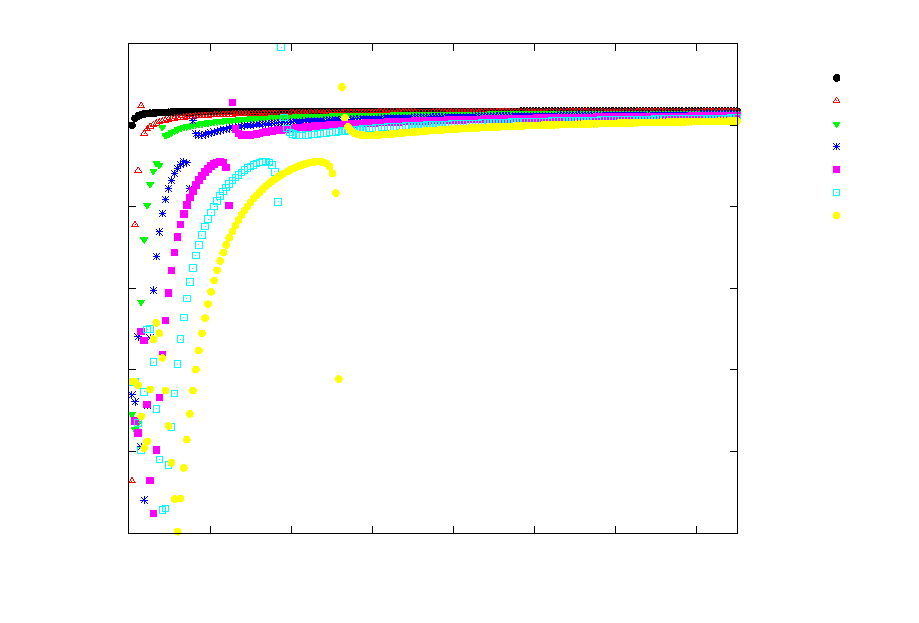
\includegraphics{tnnsmallangsize}}%
    \gplfronttext
  \end{picture}%
\endgroup

	\caption{Results for $t_0(q,q)$ with an angular grid size of $4$}
	\label{fig:tnnsmallangsize}
\end{figure}


The behaviour is qualitatively the same: at low $p_{max}$, $|t|$ rises fast from zero to a bit below $0.25\si{\femto\meter^2}$. At some points, there is what appears to be pole like behaviour, a sudden drop to zero and then again going near $0.25\si{\femto\meter^2}$ from above. For larger grid sizes, this pole is shifted to higher $p_{max}$, and the poles are also shifted towards higher $p_{max}$ for larger angular grid sizes. After the poles, $|t|$ approaches a value a bit above $0.25\si{\femto\meter^2}$, however for smaller grid sizes, this value is a  bit higher than for larger grid sizes, differing by about $2\%$, or in the third significant digit.

This is not exactly what we were expecting, we would have expected a difference that is not visible when plotting. 

Becaue the poles appear at $p_{max}$ as high as about $9000\si{\per\femto\meter}$, we choose the largest possible angular size for subsequent measurements, a grid size of $50$ and a pmax of $100000$, about seven times as high as the highest pmax we lookes at here. We hope to avoid any complications with poles this way.

\begin{figure}[htbp]
	% GNUPLOT: LaTeX picture with Postscript
\begingroup
  \makeatletter
  \providecommand\color[2][]{%
    \GenericError{(gnuplot) \space\space\space\@spaces}{%
      Package color not loaded in conjunction with
      terminal option `colourtext'%
    }{See the gnuplot documentation for explanation.%
    }{Either use 'blacktext' in gnuplot or load the package
      color.sty in LaTeX.}%
    \renewcommand\color[2][]{}%
  }%
  \providecommand\includegraphics[2][]{%
    \GenericError{(gnuplot) \space\space\space\@spaces}{%
      Package graphicx or graphics not loaded%
    }{See the gnuplot documentation for explanation.%
    }{The gnuplot epslatex terminal needs graphicx.sty or graphics.sty.}%
    \renewcommand\includegraphics[2][]{}%
  }%
  \providecommand\rotatebox[2]{#2}%
  \@ifundefined{ifGPcolor}{%
    \newif\ifGPcolor
    \GPcolortrue
  }{}%
  \@ifundefined{ifGPblacktext}{%
    \newif\ifGPblacktext
    \GPblacktextfalse
  }{}%
  % define a \g@addto@macro without @ in the name:
  \let\gplgaddtomacro\g@addto@macro
  % define empty templates for all commands taking text:
  \gdef\gplbacktext{}%
  \gdef\gplfronttext{}%
  \makeatother
  \ifGPblacktext
    % no textcolor at all
    \def\colorrgb#1{}%
    \def\colorgray#1{}%
  \else
    % gray or color?
    \ifGPcolor
      \def\colorrgb#1{\color[rgb]{#1}}%
      \def\colorgray#1{\color[gray]{#1}}%
      \expandafter\def\csname LTw\endcsname{\color{white}}%
      \expandafter\def\csname LTb\endcsname{\color{black}}%
      \expandafter\def\csname LTa\endcsname{\color{black}}%
      \expandafter\def\csname LT0\endcsname{\color[rgb]{1,0,0}}%
      \expandafter\def\csname LT1\endcsname{\color[rgb]{0,1,0}}%
      \expandafter\def\csname LT2\endcsname{\color[rgb]{0,0,1}}%
      \expandafter\def\csname LT3\endcsname{\color[rgb]{1,0,1}}%
      \expandafter\def\csname LT4\endcsname{\color[rgb]{0,1,1}}%
      \expandafter\def\csname LT5\endcsname{\color[rgb]{1,1,0}}%
      \expandafter\def\csname LT6\endcsname{\color[rgb]{0,0,0}}%
      \expandafter\def\csname LT7\endcsname{\color[rgb]{1,0.3,0}}%
      \expandafter\def\csname LT8\endcsname{\color[rgb]{0.5,0.5,0.5}}%
    \else
      % gray
      \def\colorrgb#1{\color{black}}%
      \def\colorgray#1{\color[gray]{#1}}%
      \expandafter\def\csname LTw\endcsname{\color{white}}%
      \expandafter\def\csname LTb\endcsname{\color{black}}%
      \expandafter\def\csname LTa\endcsname{\color{black}}%
      \expandafter\def\csname LT0\endcsname{\color{black}}%
      \expandafter\def\csname LT1\endcsname{\color{black}}%
      \expandafter\def\csname LT2\endcsname{\color{black}}%
      \expandafter\def\csname LT3\endcsname{\color{black}}%
      \expandafter\def\csname LT4\endcsname{\color{black}}%
      \expandafter\def\csname LT5\endcsname{\color{black}}%
      \expandafter\def\csname LT6\endcsname{\color{black}}%
      \expandafter\def\csname LT7\endcsname{\color{black}}%
      \expandafter\def\csname LT8\endcsname{\color{black}}%
    \fi
  \fi
    \setlength{\unitlength}{0.0500bp}%
    \ifx\gptboxheight\undefined%
      \newlength{\gptboxheight}%
      \newlength{\gptboxwidth}%
      \newsavebox{\gptboxtext}%
    \fi%
    \setlength{\fboxrule}{0.5pt}%
    \setlength{\fboxsep}{1pt}%
\begin{picture}(8502.00,5668.00)%
    \gplgaddtomacro\gplbacktext{%
      \csname LTb\endcsname%
      \put(946,704){\makebox(0,0)[r]{\strut{}$0$}}%
      \put(946,1487){\makebox(0,0)[r]{\strut{}$0.05$}}%
      \put(946,2270){\makebox(0,0)[r]{\strut{}$0.1$}}%
      \put(946,3054){\makebox(0,0)[r]{\strut{}$0.15$}}%
      \put(946,3837){\makebox(0,0)[r]{\strut{}$0.2$}}%
      \put(946,4620){\makebox(0,0)[r]{\strut{}$0.25$}}%
      \put(946,5403){\makebox(0,0)[r]{\strut{}$0.3$}}%
      \put(1078,484){\makebox(0,0){\strut{}$0$}}%
      \put(1857,484){\makebox(0,0){\strut{}$2000$}}%
      \put(2635,484){\makebox(0,0){\strut{}$4000$}}%
      \put(3414,484){\makebox(0,0){\strut{}$6000$}}%
      \put(4192,484){\makebox(0,0){\strut{}$8000$}}%
      \put(4971,484){\makebox(0,0){\strut{}$10000$}}%
      \put(5749,484){\makebox(0,0){\strut{}$12000$}}%
      \put(6528,484){\makebox(0,0){\strut{}$14000$}}%
    }%
    \gplgaddtomacro\gplfronttext{%
      \csname LTb\endcsname%
      \put(176,3053){\rotatebox{-270}{\makebox(0,0){\strut{}$|t_0(q,q)|/\si{\femto\meter^2}$}}}%
      \put(3997,154){\makebox(0,0){\strut{}$p_{max}/\si{\per\femto\meter}$}}%
      \put(7775,5293){\makebox(0,0){\strut{}Grid points}}%
      \csname LTb\endcsname%
      \put(7445,5073){\makebox(0,0)[r]{\strut{}4}}%
      \csname LTb\endcsname%
      \put(7445,4853){\makebox(0,0)[r]{\strut{}12}}%
      \csname LTb\endcsname%
      \put(7445,4633){\makebox(0,0)[r]{\strut{}20}}%
      \csname LTb\endcsname%
      \put(7445,4413){\makebox(0,0)[r]{\strut{}28}}%
      \csname LTb\endcsname%
      \put(7445,4193){\makebox(0,0)[r]{\strut{}36}}%
      \csname LTb\endcsname%
      \put(7445,3973){\makebox(0,0)[r]{\strut{}44}}%
      \csname LTb\endcsname%
      \put(7445,3753){\makebox(0,0)[r]{\strut{}52}}%
    }%
    \gplbacktext
    \put(0,0){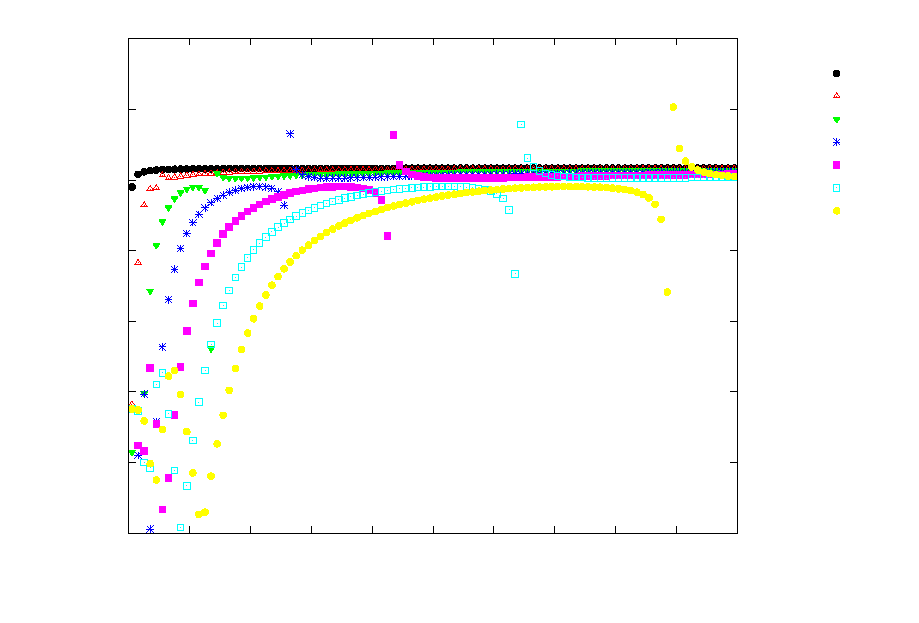
\includegraphics{tnnbigangsize}}%
    \gplfronttext
  \end{picture}%
\endgroup

	\caption{Results for $t_0(q,q)$ with an angular grid size of $60$}
	\label{fig:tnnbigangsize}
\end{figure}

We repeat our measurements, however we neglect the term $\sim \ln\left(\frac{p_{max}+q}{p_{max}-q}\right)$ in the matrix $A$. The results can be seen in fig.~\ref{fig:tnnsmallangsizewopm} and fig.~\ref{fig:tnnbigangsizewopm}. 

\begin{figure}[htbp]
	% GNUPLOT: LaTeX picture with Postscript
\begingroup
  \makeatletter
  \providecommand\color[2][]{%
    \GenericError{(gnuplot) \space\space\space\@spaces}{%
      Package color not loaded in conjunction with
      terminal option `colourtext'%
    }{See the gnuplot documentation for explanation.%
    }{Either use 'blacktext' in gnuplot or load the package
      color.sty in LaTeX.}%
    \renewcommand\color[2][]{}%
  }%
  \providecommand\includegraphics[2][]{%
    \GenericError{(gnuplot) \space\space\space\@spaces}{%
      Package graphicx or graphics not loaded%
    }{See the gnuplot documentation for explanation.%
    }{The gnuplot epslatex terminal needs graphicx.sty or graphics.sty.}%
    \renewcommand\includegraphics[2][]{}%
  }%
  \providecommand\rotatebox[2]{#2}%
  \@ifundefined{ifGPcolor}{%
    \newif\ifGPcolor
    \GPcolortrue
  }{}%
  \@ifundefined{ifGPblacktext}{%
    \newif\ifGPblacktext
    \GPblacktextfalse
  }{}%
  % define a \g@addto@macro without @ in the name:
  \let\gplgaddtomacro\g@addto@macro
  % define empty templates for all commands taking text:
  \gdef\gplbacktext{}%
  \gdef\gplfronttext{}%
  \makeatother
  \ifGPblacktext
    % no textcolor at all
    \def\colorrgb#1{}%
    \def\colorgray#1{}%
  \else
    % gray or color?
    \ifGPcolor
      \def\colorrgb#1{\color[rgb]{#1}}%
      \def\colorgray#1{\color[gray]{#1}}%
      \expandafter\def\csname LTw\endcsname{\color{white}}%
      \expandafter\def\csname LTb\endcsname{\color{black}}%
      \expandafter\def\csname LTa\endcsname{\color{black}}%
      \expandafter\def\csname LT0\endcsname{\color[rgb]{1,0,0}}%
      \expandafter\def\csname LT1\endcsname{\color[rgb]{0,1,0}}%
      \expandafter\def\csname LT2\endcsname{\color[rgb]{0,0,1}}%
      \expandafter\def\csname LT3\endcsname{\color[rgb]{1,0,1}}%
      \expandafter\def\csname LT4\endcsname{\color[rgb]{0,1,1}}%
      \expandafter\def\csname LT5\endcsname{\color[rgb]{1,1,0}}%
      \expandafter\def\csname LT6\endcsname{\color[rgb]{0,0,0}}%
      \expandafter\def\csname LT7\endcsname{\color[rgb]{1,0.3,0}}%
      \expandafter\def\csname LT8\endcsname{\color[rgb]{0.5,0.5,0.5}}%
    \else
      % gray
      \def\colorrgb#1{\color{black}}%
      \def\colorgray#1{\color[gray]{#1}}%
      \expandafter\def\csname LTw\endcsname{\color{white}}%
      \expandafter\def\csname LTb\endcsname{\color{black}}%
      \expandafter\def\csname LTa\endcsname{\color{black}}%
      \expandafter\def\csname LT0\endcsname{\color{black}}%
      \expandafter\def\csname LT1\endcsname{\color{black}}%
      \expandafter\def\csname LT2\endcsname{\color{black}}%
      \expandafter\def\csname LT3\endcsname{\color{black}}%
      \expandafter\def\csname LT4\endcsname{\color{black}}%
      \expandafter\def\csname LT5\endcsname{\color{black}}%
      \expandafter\def\csname LT6\endcsname{\color{black}}%
      \expandafter\def\csname LT7\endcsname{\color{black}}%
      \expandafter\def\csname LT8\endcsname{\color{black}}%
    \fi
  \fi
    \setlength{\unitlength}{0.0500bp}%
    \ifx\gptboxheight\undefined%
      \newlength{\gptboxheight}%
      \newlength{\gptboxwidth}%
      \newsavebox{\gptboxtext}%
    \fi%
    \setlength{\fboxrule}{0.5pt}%
    \setlength{\fboxsep}{1pt}%
\begin{picture}(8502.00,5668.00)%
    \gplgaddtomacro\gplbacktext{%
      \csname LTb\endcsname%
      \put(946,704){\makebox(0,0)[r]{\strut{}$0$}}%
      \put(946,1487){\makebox(0,0)[r]{\strut{}$0.05$}}%
      \put(946,2270){\makebox(0,0)[r]{\strut{}$0.1$}}%
      \put(946,3054){\makebox(0,0)[r]{\strut{}$0.15$}}%
      \put(946,3837){\makebox(0,0)[r]{\strut{}$0.2$}}%
      \put(946,4620){\makebox(0,0)[r]{\strut{}$0.25$}}%
      \put(946,5403){\makebox(0,0)[r]{\strut{}$0.3$}}%
      \put(1078,484){\makebox(0,0){\strut{}$0$}}%
      \put(1857,484){\makebox(0,0){\strut{}$2000$}}%
      \put(2635,484){\makebox(0,0){\strut{}$4000$}}%
      \put(3414,484){\makebox(0,0){\strut{}$6000$}}%
      \put(4192,484){\makebox(0,0){\strut{}$8000$}}%
      \put(4971,484){\makebox(0,0){\strut{}$10000$}}%
      \put(5749,484){\makebox(0,0){\strut{}$12000$}}%
      \put(6528,484){\makebox(0,0){\strut{}$14000$}}%
    }%
    \gplgaddtomacro\gplfronttext{%
      \csname LTb\endcsname%
      \put(176,3053){\rotatebox{-270}{\makebox(0,0){\strut{}$|t_0(q,q)|/\si{\femto\meter^2}$}}}%
      \put(3997,154){\makebox(0,0){\strut{}$p_{max}/\si{\per\femto\meter}$}}%
      \put(7775,5293){\makebox(0,0){\strut{}Grid points}}%
      \csname LTb\endcsname%
      \put(7445,5073){\makebox(0,0)[r]{\strut{}4}}%
      \csname LTb\endcsname%
      \put(7445,4853){\makebox(0,0)[r]{\strut{}12}}%
      \csname LTb\endcsname%
      \put(7445,4633){\makebox(0,0)[r]{\strut{}20}}%
      \csname LTb\endcsname%
      \put(7445,4413){\makebox(0,0)[r]{\strut{}28}}%
      \csname LTb\endcsname%
      \put(7445,4193){\makebox(0,0)[r]{\strut{}36}}%
      \csname LTb\endcsname%
      \put(7445,3973){\makebox(0,0)[r]{\strut{}44}}%
      \csname LTb\endcsname%
      \put(7445,3753){\makebox(0,0)[r]{\strut{}52}}%
    }%
    \gplbacktext
    \put(0,0){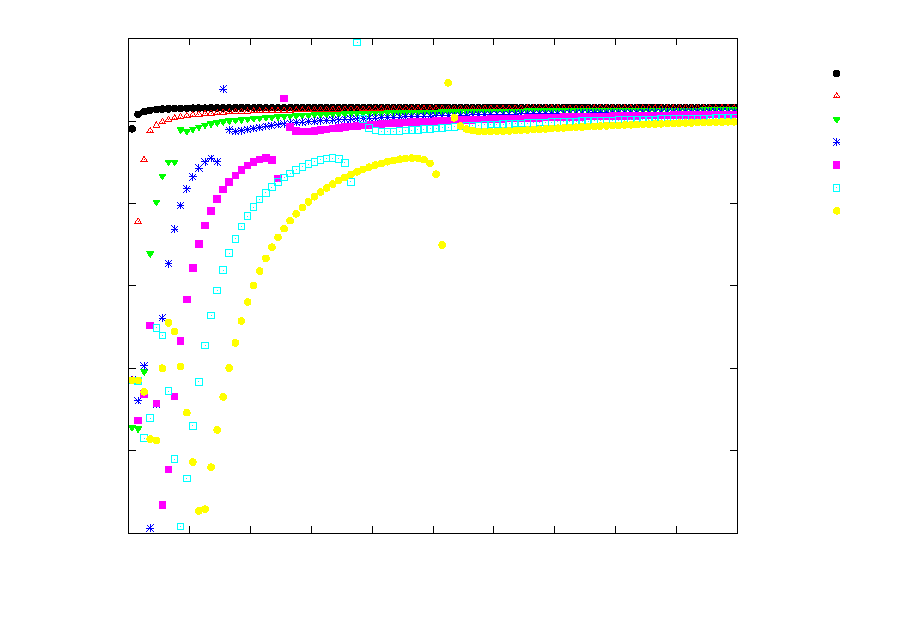
\includegraphics{tnnsmallangsizewopm}}%
    \gplfronttext
  \end{picture}%
\endgroup

	\caption{Results for $t_0(q,q)$ with an angular grid size of $4$, neglecting the term $\sim p_{max}$ in $A$}
	\label{fig:tnnsmallangsizewopm}
\end{figure}

The results look very similar to those were we did not neglect this term, and a cloeser look at our results show that the measurements indeed only differ at about the fifth significant digit. This is not so surprising, because $q=\sqrt{2\cdot1\cdot 938.92}/197.3^2=0.22\si{\per\femto\meter}$ is much smaller than any $p_{max}$ we are looking at, and so the term explicitly containing $p_{max}$ is very close to zero anyway.

\begin{figure}[htbp]
	% GNUPLOT: LaTeX picture with Postscript
\begingroup
  \makeatletter
  \providecommand\color[2][]{%
    \GenericError{(gnuplot) \space\space\space\@spaces}{%
      Package color not loaded in conjunction with
      terminal option `colourtext'%
    }{See the gnuplot documentation for explanation.%
    }{Either use 'blacktext' in gnuplot or load the package
      color.sty in LaTeX.}%
    \renewcommand\color[2][]{}%
  }%
  \providecommand\includegraphics[2][]{%
    \GenericError{(gnuplot) \space\space\space\@spaces}{%
      Package graphicx or graphics not loaded%
    }{See the gnuplot documentation for explanation.%
    }{The gnuplot epslatex terminal needs graphicx.sty or graphics.sty.}%
    \renewcommand\includegraphics[2][]{}%
  }%
  \providecommand\rotatebox[2]{#2}%
  \@ifundefined{ifGPcolor}{%
    \newif\ifGPcolor
    \GPcolortrue
  }{}%
  \@ifundefined{ifGPblacktext}{%
    \newif\ifGPblacktext
    \GPblacktextfalse
  }{}%
  % define a \g@addto@macro without @ in the name:
  \let\gplgaddtomacro\g@addto@macro
  % define empty templates for all commands taking text:
  \gdef\gplbacktext{}%
  \gdef\gplfronttext{}%
  \makeatother
  \ifGPblacktext
    % no textcolor at all
    \def\colorrgb#1{}%
    \def\colorgray#1{}%
  \else
    % gray or color?
    \ifGPcolor
      \def\colorrgb#1{\color[rgb]{#1}}%
      \def\colorgray#1{\color[gray]{#1}}%
      \expandafter\def\csname LTw\endcsname{\color{white}}%
      \expandafter\def\csname LTb\endcsname{\color{black}}%
      \expandafter\def\csname LTa\endcsname{\color{black}}%
      \expandafter\def\csname LT0\endcsname{\color[rgb]{1,0,0}}%
      \expandafter\def\csname LT1\endcsname{\color[rgb]{0,1,0}}%
      \expandafter\def\csname LT2\endcsname{\color[rgb]{0,0,1}}%
      \expandafter\def\csname LT3\endcsname{\color[rgb]{1,0,1}}%
      \expandafter\def\csname LT4\endcsname{\color[rgb]{0,1,1}}%
      \expandafter\def\csname LT5\endcsname{\color[rgb]{1,1,0}}%
      \expandafter\def\csname LT6\endcsname{\color[rgb]{0,0,0}}%
      \expandafter\def\csname LT7\endcsname{\color[rgb]{1,0.3,0}}%
      \expandafter\def\csname LT8\endcsname{\color[rgb]{0.5,0.5,0.5}}%
    \else
      % gray
      \def\colorrgb#1{\color{black}}%
      \def\colorgray#1{\color[gray]{#1}}%
      \expandafter\def\csname LTw\endcsname{\color{white}}%
      \expandafter\def\csname LTb\endcsname{\color{black}}%
      \expandafter\def\csname LTa\endcsname{\color{black}}%
      \expandafter\def\csname LT0\endcsname{\color{black}}%
      \expandafter\def\csname LT1\endcsname{\color{black}}%
      \expandafter\def\csname LT2\endcsname{\color{black}}%
      \expandafter\def\csname LT3\endcsname{\color{black}}%
      \expandafter\def\csname LT4\endcsname{\color{black}}%
      \expandafter\def\csname LT5\endcsname{\color{black}}%
      \expandafter\def\csname LT6\endcsname{\color{black}}%
      \expandafter\def\csname LT7\endcsname{\color{black}}%
      \expandafter\def\csname LT8\endcsname{\color{black}}%
    \fi
  \fi
    \setlength{\unitlength}{0.0500bp}%
    \ifx\gptboxheight\undefined%
      \newlength{\gptboxheight}%
      \newlength{\gptboxwidth}%
      \newsavebox{\gptboxtext}%
    \fi%
    \setlength{\fboxrule}{0.5pt}%
    \setlength{\fboxsep}{1pt}%
\begin{picture}(8502.00,5668.00)%
    \gplgaddtomacro\gplbacktext{%
      \csname LTb\endcsname%
      \put(946,704){\makebox(0,0)[r]{\strut{}$0$}}%
      \put(946,1375){\makebox(0,0)[r]{\strut{}$0.05$}}%
      \put(946,2047){\makebox(0,0)[r]{\strut{}$0.1$}}%
      \put(946,2718){\makebox(0,0)[r]{\strut{}$0.15$}}%
      \put(946,3389){\makebox(0,0)[r]{\strut{}$0.2$}}%
      \put(946,4060){\makebox(0,0)[r]{\strut{}$0.25$}}%
      \put(946,4732){\makebox(0,0)[r]{\strut{}$0.3$}}%
      \put(946,5403){\makebox(0,0)[r]{\strut{}$0.35$}}%
      \put(1078,484){\makebox(0,0){\strut{}$0$}}%
      \put(1662,484){\makebox(0,0){\strut{}$1000$}}%
      \put(2246,484){\makebox(0,0){\strut{}$2000$}}%
      \put(2830,484){\makebox(0,0){\strut{}$3000$}}%
      \put(3414,484){\makebox(0,0){\strut{}$4000$}}%
      \put(3998,484){\makebox(0,0){\strut{}$5000$}}%
      \put(4581,484){\makebox(0,0){\strut{}$6000$}}%
      \put(5165,484){\makebox(0,0){\strut{}$7000$}}%
      \put(5749,484){\makebox(0,0){\strut{}$8000$}}%
      \put(6333,484){\makebox(0,0){\strut{}$9000$}}%
      \put(6917,484){\makebox(0,0){\strut{}$10000$}}%
    }%
    \gplgaddtomacro\gplfronttext{%
      \csname LTb\endcsname%
      \put(176,3053){\rotatebox{-270}{\makebox(0,0){\strut{}$|t_0(q,q)|/\si{\femto\meter^2}$}}}%
      \put(3997,154){\makebox(0,0){\strut{}$p_{max}/\si{\per\femto\meter}$}}%
      \put(7775,5293){\makebox(0,0){\strut{}Grid points}}%
      \csname LTb\endcsname%
      \put(7445,5073){\makebox(0,0)[r]{\strut{}4}}%
      \csname LTb\endcsname%
      \put(7445,4853){\makebox(0,0)[r]{\strut{}12}}%
      \csname LTb\endcsname%
      \put(7445,4633){\makebox(0,0)[r]{\strut{}20}}%
      \csname LTb\endcsname%
      \put(7445,4413){\makebox(0,0)[r]{\strut{}28}}%
      \csname LTb\endcsname%
      \put(7445,4193){\makebox(0,0)[r]{\strut{}36}}%
      \csname LTb\endcsname%
      \put(7445,3973){\makebox(0,0)[r]{\strut{}44}}%
      \csname LTb\endcsname%
      \put(7445,3753){\makebox(0,0)[r]{\strut{}52}}%
    }%
    \gplbacktext
    \put(0,0){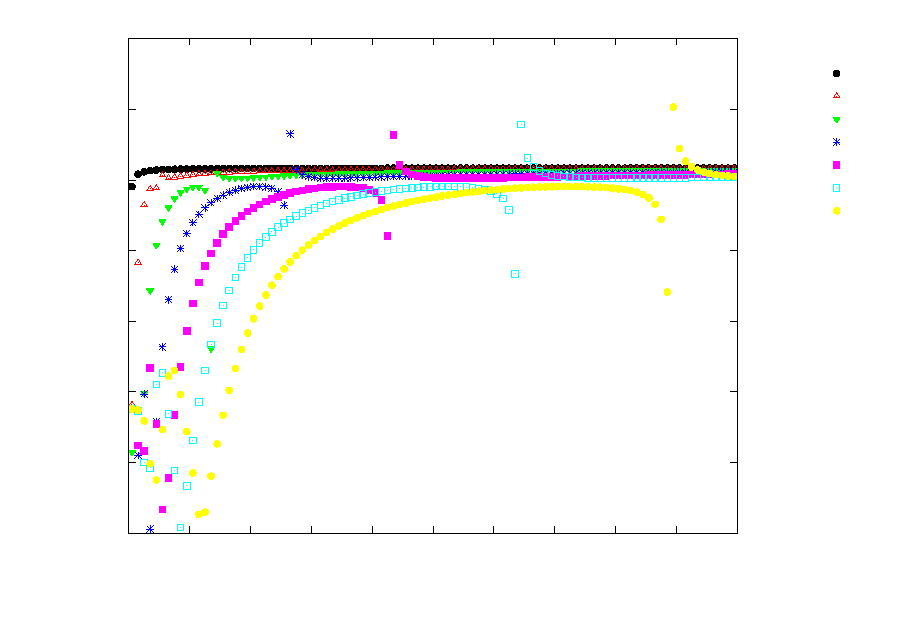
\includegraphics{tnnbigangsizewopm}}%
    \gplfronttext
  \end{picture}%
\endgroup

	\caption{Results for $t_0(q,q)$ with an angular grid size of $60$, neglecting the term $\sim p_{max}$ in $A$}
	\label{fig:tnnbigangsizewopm}
\end{figure}

\subsection{$|S|$ and $\delta_0(q)$}
We calculate $|S_0(q)|-1$ with the function \texttt{gsl\_complex\_abs} and see that for all $q$ we look at, this is either 0 or in the order of magnitude of $10^{-16}$, so in the order of numerical accuracy of a computer. So our values for $S$ reproduce the desired properties. 

The phase of $\delta(q)$ is plotted in fig.~\ref{fig:delta}.

The phase returned by the gsl-function is in the region $-\pi<\phi<\pi$, corresponding to $-\pi/2<\delta<\pi/2$. This reproduces the behaviour we want ($\delta\to 0$ for $E\to\infty$) very well, so we do not need to introduce additional factors of $\pi/2$. We see that there is a steep rise from $\delta(0)=0$ to $\delta(q=0.5\si{\per\femto\meter})=3\pi/8$, where the maximum is reached. After that, $\delta$ gets monotonously smaller and reaches $\delta(q=3.11\si{\per\femto\meter})=0.2\pi$.

\begin{figure}[htbp]
	% GNUPLOT: LaTeX picture with Postscript
\begingroup
  \makeatletter
  \providecommand\color[2][]{%
    \GenericError{(gnuplot) \space\space\space\@spaces}{%
      Package color not loaded in conjunction with
      terminal option `colourtext'%
    }{See the gnuplot documentation for explanation.%
    }{Either use 'blacktext' in gnuplot or load the package
      color.sty in LaTeX.}%
    \renewcommand\color[2][]{}%
  }%
  \providecommand\includegraphics[2][]{%
    \GenericError{(gnuplot) \space\space\space\@spaces}{%
      Package graphicx or graphics not loaded%
    }{See the gnuplot documentation for explanation.%
    }{The gnuplot epslatex terminal needs graphicx.sty or graphics.sty.}%
    \renewcommand\includegraphics[2][]{}%
  }%
  \providecommand\rotatebox[2]{#2}%
  \@ifundefined{ifGPcolor}{%
    \newif\ifGPcolor
    \GPcolortrue
  }{}%
  \@ifundefined{ifGPblacktext}{%
    \newif\ifGPblacktext
    \GPblacktextfalse
  }{}%
  % define a \g@addto@macro without @ in the name:
  \let\gplgaddtomacro\g@addto@macro
  % define empty templates for all commands taking text:
  \gdef\gplbacktext{}%
  \gdef\gplfronttext{}%
  \makeatother
  \ifGPblacktext
    % no textcolor at all
    \def\colorrgb#1{}%
    \def\colorgray#1{}%
  \else
    % gray or color?
    \ifGPcolor
      \def\colorrgb#1{\color[rgb]{#1}}%
      \def\colorgray#1{\color[gray]{#1}}%
      \expandafter\def\csname LTw\endcsname{\color{white}}%
      \expandafter\def\csname LTb\endcsname{\color{black}}%
      \expandafter\def\csname LTa\endcsname{\color{black}}%
      \expandafter\def\csname LT0\endcsname{\color[rgb]{1,0,0}}%
      \expandafter\def\csname LT1\endcsname{\color[rgb]{0,1,0}}%
      \expandafter\def\csname LT2\endcsname{\color[rgb]{0,0,1}}%
      \expandafter\def\csname LT3\endcsname{\color[rgb]{1,0,1}}%
      \expandafter\def\csname LT4\endcsname{\color[rgb]{0,1,1}}%
      \expandafter\def\csname LT5\endcsname{\color[rgb]{1,1,0}}%
      \expandafter\def\csname LT6\endcsname{\color[rgb]{0,0,0}}%
      \expandafter\def\csname LT7\endcsname{\color[rgb]{1,0.3,0}}%
      \expandafter\def\csname LT8\endcsname{\color[rgb]{0.5,0.5,0.5}}%
    \else
      % gray
      \def\colorrgb#1{\color{black}}%
      \def\colorgray#1{\color[gray]{#1}}%
      \expandafter\def\csname LTw\endcsname{\color{white}}%
      \expandafter\def\csname LTb\endcsname{\color{black}}%
      \expandafter\def\csname LTa\endcsname{\color{black}}%
      \expandafter\def\csname LT0\endcsname{\color{black}}%
      \expandafter\def\csname LT1\endcsname{\color{black}}%
      \expandafter\def\csname LT2\endcsname{\color{black}}%
      \expandafter\def\csname LT3\endcsname{\color{black}}%
      \expandafter\def\csname LT4\endcsname{\color{black}}%
      \expandafter\def\csname LT5\endcsname{\color{black}}%
      \expandafter\def\csname LT6\endcsname{\color{black}}%
      \expandafter\def\csname LT7\endcsname{\color{black}}%
      \expandafter\def\csname LT8\endcsname{\color{black}}%
    \fi
  \fi
    \setlength{\unitlength}{0.0500bp}%
    \ifx\gptboxheight\undefined%
      \newlength{\gptboxheight}%
      \newlength{\gptboxwidth}%
      \newsavebox{\gptboxtext}%
    \fi%
    \setlength{\fboxrule}{0.5pt}%
    \setlength{\fboxsep}{1pt}%
\begin{picture}(8502.00,5668.00)%
    \gplgaddtomacro\gplbacktext{%
      \csname LTb\endcsname%
      \put(946,2270){\makebox(0,0)[r]{\strut{}$\pi/8$}}%
      \put(946,3837){\makebox(0,0)[r]{\strut{}$\pi/4$}}%
      \put(946,5403){\makebox(0,0)[r]{\strut{}$3\pi/8$}}%
      \put(1078,484){\makebox(0,0){\strut{}$0$}}%
      \put(2209,484){\makebox(0,0){\strut{}$0.5$}}%
      \put(3340,484){\makebox(0,0){\strut{}$1$}}%
      \put(4471,484){\makebox(0,0){\strut{}$1.5$}}%
      \put(5603,484){\makebox(0,0){\strut{}$2$}}%
      \put(6734,484){\makebox(0,0){\strut{}$2.5$}}%
      \put(7865,484){\makebox(0,0){\strut{}$3$}}%
    }%
    \gplgaddtomacro\gplfronttext{%
      \csname LTb\endcsname%
      \put(176,3053){\rotatebox{-270}{\makebox(0,0){\strut{}$\delta(q)$}}}%
      \put(4591,154){\makebox(0,0){\strut{}$q/\si{\per\femto\meter}$}}%
      \put(7545,5230){\makebox(0,0){\strut{}}}%
    }%
    \gplbacktext
    \put(0,0){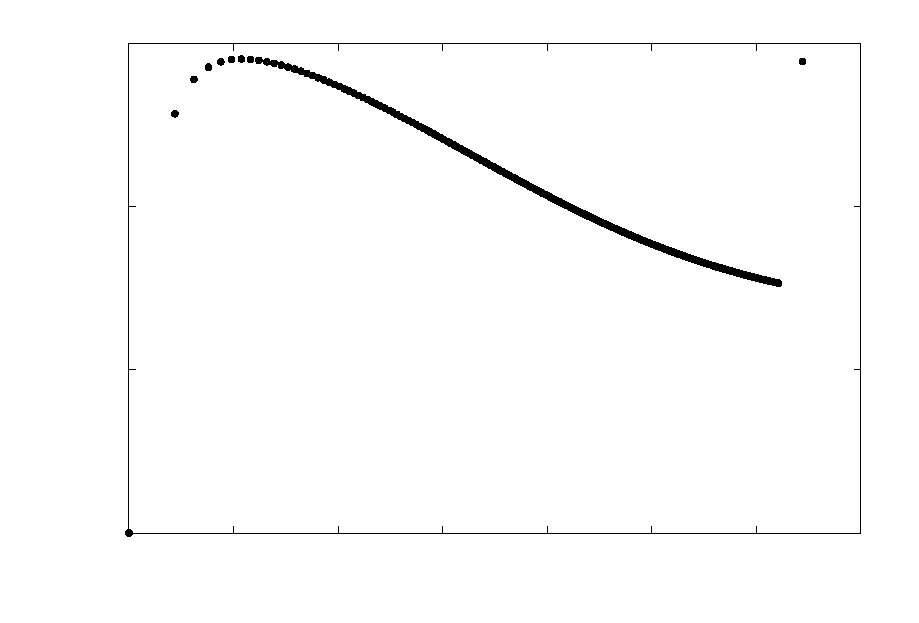
\includegraphics{delta}}%
    \gplfronttext
  \end{picture}%
\endgroup

	\caption{The phase of $S$ for different energies/$q$}
	\label{fig:delta}
\end{figure}

\subsection{Cross section}

\begin{figure}[htbp]
	% GNUPLOT: LaTeX picture with Postscript
\begingroup
  \makeatletter
  \providecommand\color[2][]{%
    \GenericError{(gnuplot) \space\space\space\@spaces}{%
      Package color not loaded in conjunction with
      terminal option `colourtext'%
    }{See the gnuplot documentation for explanation.%
    }{Either use 'blacktext' in gnuplot or load the package
      color.sty in LaTeX.}%
    \renewcommand\color[2][]{}%
  }%
  \providecommand\includegraphics[2][]{%
    \GenericError{(gnuplot) \space\space\space\@spaces}{%
      Package graphicx or graphics not loaded%
    }{See the gnuplot documentation for explanation.%
    }{The gnuplot epslatex terminal needs graphicx.sty or graphics.sty.}%
    \renewcommand\includegraphics[2][]{}%
  }%
  \providecommand\rotatebox[2]{#2}%
  \@ifundefined{ifGPcolor}{%
    \newif\ifGPcolor
    \GPcolortrue
  }{}%
  \@ifundefined{ifGPblacktext}{%
    \newif\ifGPblacktext
    \GPblacktextfalse
  }{}%
  % define a \g@addto@macro without @ in the name:
  \let\gplgaddtomacro\g@addto@macro
  % define empty templates for all commands taking text:
  \gdef\gplbacktext{}%
  \gdef\gplfronttext{}%
  \makeatother
  \ifGPblacktext
    % no textcolor at all
    \def\colorrgb#1{}%
    \def\colorgray#1{}%
  \else
    % gray or color?
    \ifGPcolor
      \def\colorrgb#1{\color[rgb]{#1}}%
      \def\colorgray#1{\color[gray]{#1}}%
      \expandafter\def\csname LTw\endcsname{\color{white}}%
      \expandafter\def\csname LTb\endcsname{\color{black}}%
      \expandafter\def\csname LTa\endcsname{\color{black}}%
      \expandafter\def\csname LT0\endcsname{\color[rgb]{1,0,0}}%
      \expandafter\def\csname LT1\endcsname{\color[rgb]{0,1,0}}%
      \expandafter\def\csname LT2\endcsname{\color[rgb]{0,0,1}}%
      \expandafter\def\csname LT3\endcsname{\color[rgb]{1,0,1}}%
      \expandafter\def\csname LT4\endcsname{\color[rgb]{0,1,1}}%
      \expandafter\def\csname LT5\endcsname{\color[rgb]{1,1,0}}%
      \expandafter\def\csname LT6\endcsname{\color[rgb]{0,0,0}}%
      \expandafter\def\csname LT7\endcsname{\color[rgb]{1,0.3,0}}%
      \expandafter\def\csname LT8\endcsname{\color[rgb]{0.5,0.5,0.5}}%
    \else
      % gray
      \def\colorrgb#1{\color{black}}%
      \def\colorgray#1{\color[gray]{#1}}%
      \expandafter\def\csname LTw\endcsname{\color{white}}%
      \expandafter\def\csname LTb\endcsname{\color{black}}%
      \expandafter\def\csname LTa\endcsname{\color{black}}%
      \expandafter\def\csname LT0\endcsname{\color{black}}%
      \expandafter\def\csname LT1\endcsname{\color{black}}%
      \expandafter\def\csname LT2\endcsname{\color{black}}%
      \expandafter\def\csname LT3\endcsname{\color{black}}%
      \expandafter\def\csname LT4\endcsname{\color{black}}%
      \expandafter\def\csname LT5\endcsname{\color{black}}%
      \expandafter\def\csname LT6\endcsname{\color{black}}%
      \expandafter\def\csname LT7\endcsname{\color{black}}%
      \expandafter\def\csname LT8\endcsname{\color{black}}%
    \fi
  \fi
    \setlength{\unitlength}{0.0500bp}%
    \ifx\gptboxheight\undefined%
      \newlength{\gptboxheight}%
      \newlength{\gptboxwidth}%
      \newsavebox{\gptboxtext}%
    \fi%
    \setlength{\fboxrule}{0.5pt}%
    \setlength{\fboxsep}{1pt}%
\begin{picture}(8502.00,5668.00)%
    \gplgaddtomacro\gplbacktext{%
      \csname LTb\endcsname%%
      \put(396,484){\makebox(0,0){\strut{}$-1$}}%
      \put(1167,484){\makebox(0,0){\strut{}$-0.8$}}%
      \put(1938,484){\makebox(0,0){\strut{}$-0.6$}}%
      \put(2709,484){\makebox(0,0){\strut{}$-0.4$}}%
      \put(3480,484){\makebox(0,0){\strut{}$-0.2$}}%
      \put(4251,484){\makebox(0,0){\strut{}$0$}}%
      \put(5021,484){\makebox(0,0){\strut{}$0.2$}}%
      \put(5792,484){\makebox(0,0){\strut{}$0.4$}}%
      \put(6563,484){\makebox(0,0){\strut{}$0.6$}}%
      \put(7334,484){\makebox(0,0){\strut{}$0.8$}}%
      \put(8105,484){\makebox(0,0){\strut{}$1$}}%
    }%
    \gplgaddtomacro\gplfronttext{%
      \csname LTb\endcsname%%
      \put(198,3075){\rotatebox{-270}{\makebox(0,0){\strut{}$\derivative{\sigma}{\hat{q}_f}/\si{\femto\meter^2\mega\electronvolt}$}}}%
      \put(4250,154){\makebox(0,0){\strut{}$x$}}%
      \put(1021,5274){\makebox(0,0){\strut{}l=}}%
      \csname LTb\endcsname%%
      \put(660,5054){\makebox(0,0)[r]{\strut{}0}}%
      \csname LTb\endcsname%%
      \put(660,4834){\makebox(0,0)[r]{\strut{}1}}%
      \csname LTb\endcsname%%
      \put(660,4614){\makebox(0,0)[r]{\strut{}2}}%
      \csname LTb\endcsname%%
      \put(660,4394){\makebox(0,0)[r]{\strut{}3}}%
      \csname LTb\endcsname%%
      \put(660,4174){\makebox(0,0)[r]{\strut{}4}}%
      \csname LTb\endcsname%%
      \put(660,3954){\makebox(0,0)[r]{\strut{}5}}%
      \csname LTb\endcsname%%
      \put(660,3734){\makebox(0,0)[r]{\strut{}6}}%
    }%
    \gplbacktext
    \put(0,0){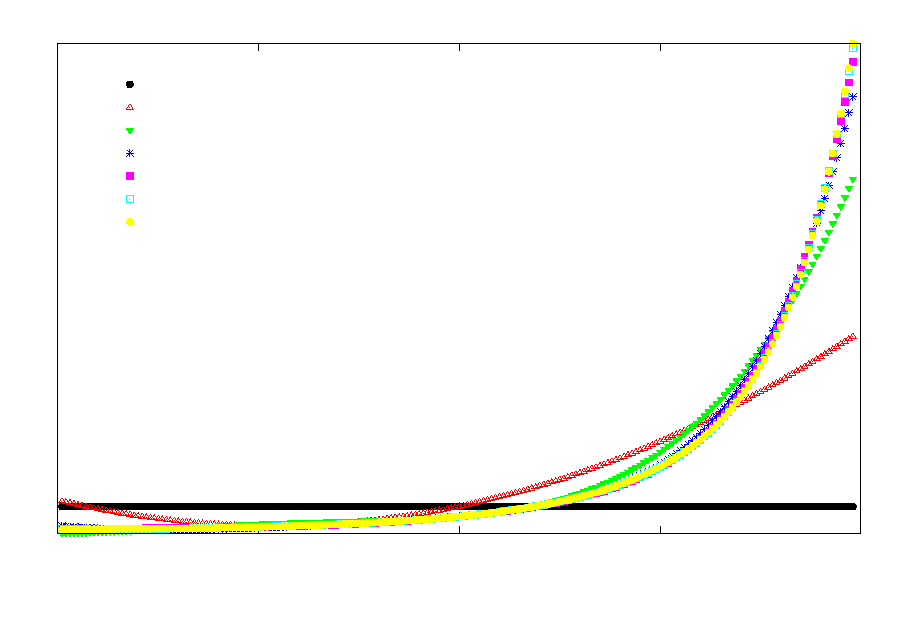
\includegraphics{crossect}}%
    \gplfronttext
  \end{picture}%
\endgroup

	\caption{The differential cross section for different $l$}
	\label{fig:crossect}
\end{figure}
As expected the cross section, shown in fig. \ref{fig:crossect}, is peaked at $x=1$, because this corresponds to $\Theta=0$. Furthermore only after summation of up to $l=2$ or higher a good approximation is reached. For $l=0$ the differential cross section is constant, because $P_0=\text{const}$.
\newpage
\listoffigures
\listoftables
\printbibliography
\end{document}
